\documentclass[10pt]{beamer}
\usepackage[T1,T2A]{fontenc}
\usepackage[utf8]{inputenc}
\usepackage{hyperref}
\hypersetup{unicode=true}
\usepackage{fontawesome}
\usepackage{graphicx}
\usepackage[english,russian]{babel}

\usepackage[T1]{fontenc}
\usepackage{fontawesome}
\usepackage{PTSans} 
\mode<presentation>
{
  \usetheme[progressbar=foot,numbering=fraction,background=light]{metropolis} 
  \usecolortheme{default}
  \usefonttheme{default}
  \setbeamertemplate{navigation symbols}{}
  \setbeamertemplate{caption}[numbered]
} 

\let\textttorig\texttt
\renewcommand<>{\texttt}[1]{%
  \only#2{\textttorig{#1}}%
}

\usepackage{minted}

\usepackage{xcolor}
\definecolor{codecolor}{HTML}{FFC300}

\usepackage{tcolorbox}
\tcbuselibrary{most,listingsutf8,minted}

\tcbset{tcbox width=auto,left=1mm,top=1mm,bottom=1mm,
right=1mm,boxsep=1mm,middle=1pt}

\newtcblisting{myr}[1]{colback=codecolor!5,colframe=codecolor!80!black,listing only, 
minted options={numbers=left, style=tcblatex,fontsize=\tiny,breaklines,autogobble,linenos,numbersep=3mm},
left=5mm,enhanced,
title=#1, fonttitle=\bfseries,
listing engine=minted,minted language=r}

\definecolor{mygreen}{HTML}{37980D}
\definecolor{myblue}{HTML}{0D089F}
\definecolor{myred}{HTML}{98290D}

\usepackage{listings}

\lstdefinelanguage{XML}
{
  morestring=[b]",
  morecomment=[s]{<!--}{-->},
  morestring=[s]{>}{<},
  morekeywords={ref,xmlns,version,type,canonicalRef,metr,real,target}
}

\lstdefinestyle{myxml}{
language=XML,
showspaces=false,
showtabs=false,
basicstyle=\ttfamily,
columns=fullflexible,
breaklines=true,
showstringspaces=false,
breakatwhitespace=true,
escapeinside={(*@}{@*)},
basicstyle=\color{mygreen}\ttfamily,
stringstyle=\color{myred},
commentstyle=\color{myblue}\upshape,
keywordstyle=\color{myblue}\bfseries,
}


% ------------------------------------------------------------------------------
% The Document
% ------------------------------------------------------------------------------
\title{Разработка игрового приложения <<Судоку>>}
\subtitle{Отчет о проектной работе по курсу <<Основы информатики и программирования>>}
\author{А. С. Мнавер}
\date{11 июня 2021}

\begin{document}

\maketitle

\begin{frame}{Введение}
   Судоку — это головоломка, которая завоевала мировую популярность с 2005 года. Для того, чтобы решить судоку, нужны только логика и метод проб и ошибок. 
   В данном проекте речь пойдет о создании игровой программы «Судоку», которая и будет являться объектом моей работы.
\end{frame}

\begin{frame}
  \frametitle{Цель и задачи проекта}
    \begin{block}{Цель проекта:}
        разработать игровое приложение, которое реализует игру «Судоку» на языке С++ .
  \end{block}
  \begin{block}{Задачи проекта:}
  \begin{itemize}
    \item реализовать графический интерфейс пользователя.
    \item реализовать алгоритм генерации случайного игрового поля судоку.
    \item реализовать алгоритм решения произвольного игрового поля.
  \end{itemize}
  \end{block}
\end{frame}

\begin{frame}{План разработки игры}
    \begin{enumerate}
         \item Разработка модуля для игрового поля.
         \item Разработка модуля для правильной расстановки цифр от 1 до 9.
         \item Разработка модуля создания новой игры.
         \item Разработка модуля просмотра правильного решения головоломки.
         \item Разработка модуля создания время решения игры.
    \end{enumerate}
\end{frame}

\begin{frame}{mainwindow.cpp}
    \begin{itemize}
         \item реализован следующий модуль: создание новой игра --- on-New-Game-clicked(), и создание Таймера --- timerstart(); и просмотра правильного решенияголоволомки --- on-Solve-clicked() , и правильной расстановки цифр от 1 до 9 --- on-table-cellClicked(int row, int column) click-on(int num) . 
         \item А также получение изменение цвет ячейки (QColor).
    \end{itemize}
\end{frame}

\begin{frame}{matrix.cpp}
    \begin{itemize}
        \item реализовать алгоритм игрового поля new-puzzle()
        \item реализовать алгоритм решение игру solve() , dfs() , init() .
        \item проверка на победа в игре you-win()
        
    \end{itemize}
\end{frame}

\begin{frame}{mainwindow.ui}
    mainwindow.ui является главным модулем графического интерфейса, который содержит:
    \begin{enumerate}
        \item игровое поле QTablewidget.
        \item кнопки New Game и Solve и Reset и Quit .
        \item кнопки цифр от 1 до 9.
        \item timer (QLCDNumber).
    \end{enumerate}
\end{frame}

\begin{frame}{Реализация приложения}
        \begin{columns}[T,onlytextwidth]
                \begin{column}{0.44\textwidth}
                        \begin{itemize}
                                \item Для этого были использованы языки <<С++>>.
                        \end{itemize}
                \end{column}
                \begin{column}{0.45\textwidth}
                        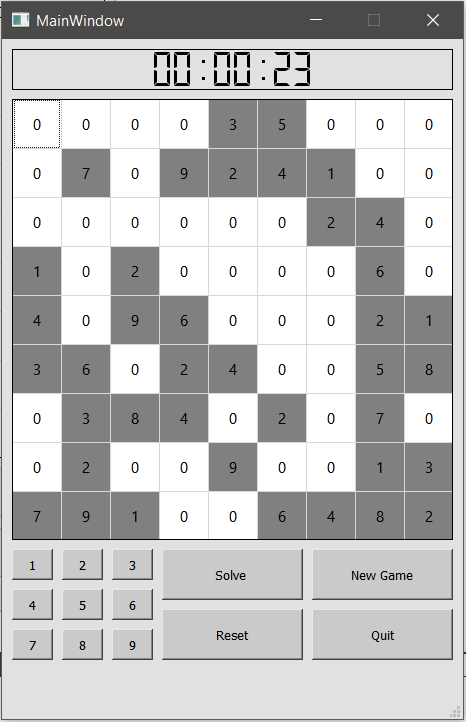
\includegraphics[width=\textwidth]{Sudoku-photo.PNG}
                \end{column}
        \end{columns}
\end{frame}

\begin{frame}
    \frametitle{Заключение}
     
    \item В ходе выполнения проектонй работы были полностью реализованы поставленные цели и задачи.  
    \item Игра имеет:
    \item графический интерфейс пользователя.
    \item Алгоритм решения произвольного игрового поля и уже заданной игры судоку. 
    \item Алгоритм генерации случайного игрового поля судоку.

\end{frame}

\begin{frame}[standout]
    Спасибо за внимание !
\end{frame}

\end{document}
